\documentclass[UserManual.tex]{subfiles}
\begin{document}
\setcounter{section}{8}

\section{Underlying Theory of {\it Smooth Emulator}}\label{sec:theory}

The choice of model emulators, $E(\vec{\theta})$, depends on the prior understanding of the model being emulated, $M(\vec{\theta})$. If one knows that  a function is linear, then a linear fit is clearly the best choice. Whereas to reproduce lumpy features, where the lumps have a characteristic length scale, Gaussian process emulators are highly effective. The quality of an emulator can be assessed through the following criteria:
\begin{itemize}
  \item $E(\vec{\theta}_t)=M(\vec{\theta}_t)$ at the training points, $\vec{\theta}_t$. 
  \item The emulator should reasonably reproduce the model away from the training points. This should hold true for either interpolation or extrapolation.
  \item The emulator should reasonably represent its uncertainty
  \item A minimal number of training points should be needed
  \item The method should easily adjust to larger numbers of parameters, $\theta_i,~i=1\cdots N$
  \item The emulator should not be affected by unitary transformations of the parameter space
  \item The emulator should be able to account for noisy models
  \item Training and running the emulator should not be numerically intensive
\end{itemize}

Here the goal is to focus on a particular class of functions: functions that are {\it smooth}. Smoothness is a prior knowledge of the function. It is an expectation that the linear terms of the function are likely to provide more variance than the quadratic contributions, which are in turn likely to be more important than the cubic corrections, and so on. 

\subsection{Mathematical Form of {\it Smooth Emulator}}

To that end the following form for $E(\vec{\theta})$ is chosen,
\begin{align*}\eqnumber\label{eq:emudef}
E(\vec{\theta})&=\sum_{\vec{n}, {\rm s.t.}~K(\vec{n})\le K_{\rm max}} d_{\vec{n}}
f_{K(\vec{n})}(|\vec{\theta}|)
A_{\vec{n}}
\left(\frac{\theta_1}{\Lambda}\right)^{n_1}\left(\frac{\theta_2}{\Lambda}\right)^{n_2}\cdots 
\left(\frac{\theta_N}{\Lambda}\right)^{n_N}.
\end{align*}
Each term has a rank $K(\vec{n})=n_1+n_2+\cdots n_N$. If $f$ is constant, the rank of that term corresponds to the power of $|\vec{\theta}|/\Lambda$. All terms are included up to a given rank, $K_{\rm max}$. The coefficients $A$ are stochastically distributed. The coefficients $d_{\vec{n}}$ will ensure that the variance is independent of the direction of $\vec{\theta}$, with the constraint that $d_{K,0,0\cdots}=1$. The function $f_K(|\vec{\theta}|)$ provides the freedom to alter how the behavior depends on the distance from the origin, $|\vec{\theta}|$, and on the rank, $K$. Given that the variance of $A_{\vec{n}}$ can be changed, $f_{K=0}(|\vec{\theta}|=0)$ is also set to unity for all $K$ without loss of generality. For each combination $\vec{n}$, the prior probability for any the $A$ coefficients is given by 
\begin{align*}\eqnumber
p(A_{\vec{n}})&=\frac{1}{\sqrt{2\pi\sigma^2_{K(\vec{n})}}} e^{-A_{\vec{n}}^2/2\sigma_{K(\vec{n})}^2},\\
\langle A^2_{\vec{n}}\rangle&=\sigma^2_{K(\vec{n})}.
\end{align*}
The variance, $\sigma^2_K$, is allowed to vary as a function of $K$.

The parameter $\Lambda$ will be referred to as the {\it smoothness parameter}. Here, we assume that all parameters have a similar range, of order unity, e.g. $-1<\theta_i<1$. Thus, the relative importance of each term Eq. (\ref{eq:emudef}) falls with increasing rank, $K$, as $(1/\Lambda)^K$. For now, the smoothness parameter is fixed by prior knowledge, i.e. one chooses higher values of $\Lambda$ if one believes the function to be close to linear.

First, we consider the variance of the emulator at a given point, $\vec{\theta}$. Requiring that the variance is independent of the direction of $\vec{\theta}$ will fix $d_{\vec{n}}$.  For example, transforming $\theta_1$ and $\theta_2$ to parameters $(\theta_1\pm\theta_2)/\sqrt{2}$ should not affect the accuracy or uncertainty of the emulator.

At $|\vec{\theta}|=0$ the only term in Eq. (\ref{eq:emudef}) that contributes to the variance is the one $K=0$ term. Averaging over the $A$ coefficients, which can be either positive or negative with equal probability,
\begin{align*}\eqnumber
\langle E(\vec{\theta})\rangle=0,
\end{align*}
where the averaging refers to an average over the $A$ coefficients. At the origin, $|\vec{\theta}|=0$, the variance of $E$ is
\begin{align*}\eqnumber
\langle E(\theta_1=\theta_2=\cdots\theta_N=0)^2\rangle=d^2_{n_i=0}\sigma_{K=0}^2f_{K=0}^2(\vec{\theta}=0).
\end{align*}
Choosing $f_{K=0}(0)=1$ and $d_{n_i=0}=1$, the variance of $E$ is indeed $\sigma_0^2$. 
The variance at some point $\vec{\theta}\ne 0$ is 
\begin{align*}\eqnumber
\langle E^2(\vec{\theta})\rangle &=
\sum_{\vec{n}} 
f_K^2(|\vec{\theta}|)\sigma^2_{K(\vec{n})} d_{\vec{n}}^2
\left(\frac{\theta_1^{2n_1}}{\Lambda^2}\right)\left(\frac{\theta_2^{2n_2}}{\Lambda^2}\right)\cdots 
\left(\frac{\theta_N^{2n_N}}{\Lambda^2}\right).
\end{align*}
If $\langle E^2\rangle$ is to be independent of the direction of $\vec{\theta}$, the sum above must be a function of $|\vec{\theta}|^2$ only. This requires the net contribution from each rank, $K$ to be proportional to  $|\vec{\theta}|^{2K}$ multiplied by some function of $K$. Using the fact that
\begin{align*}\eqnumber
(\vec{\theta}_a\cdot \vec{\theta}_b)^K&=\sum_{\vec{n},s.t. \sum_i n_i=K}\frac{K!}{n_1!\cdots n_N!}(\theta_{a1}\theta_{b1})^{n_1}\cdots(\theta_{aN}\theta_{bN})^{n_N},
\end{align*}
one can see that if the sum is to depend only on the norm of $\vec{\theta}$,
\begin{align*}\eqnumber
d_{\vec{n}}^2&=\frac{K(\vec{n})!}{n_1!n_2!\cdots n_N!}.
\end{align*}
The factor of $K!$ in the numerator was chosen to satisfy the condition that $d_{K,0,0,0}=1$.

One can now calculate the correlation between the emulator at two different points, averaged over all possible values of $A$,
\begin{align*}\eqnumber
\langle E(\vec{\theta}_a)E(\vec{\theta}_b)\rangle &=
\sum_{K=0}^{K_{\rm max}}\sigma_K^2f_K^2(|\vec{\theta}|)
\left(\frac{\vec{\theta}_a\cdot\vec{\theta}_b}{\Lambda^2}\right)^{K}.
\end{align*}
Requiring $f(|\theta|=0)=1$ gives
\begin{align*}\eqnumber
\langle E^2(\vec{\theta}=0))\rangle &=\sigma_0^2,
\end{align*}
and for $\vec{\theta}_a=\vec{\theta}_b$,
\begin{eqnarray}
\langle E^2(\vec{\theta}=0))\rangle &=\sum_{K=0}^{K_{\rm max}}
\sigma_K^2f_K^2(|\vec{\theta}|)\left(\frac{|\vec{\theta}|^2}{\Lambda^2}\right)^K.
\end{eqnarray}

To this point, the form is completely general once one requires that the variance above is independent of the direction of $\vec{\theta}$. I.e. the function $f_K(\vec{\theta})$ could be any function satisfying the constraint, $f_K(0)=1$, and $\sigma_K^2$ could have any function of $K$. Below, we illustrate how different choices for $f$ or for $\sigma_K$ affect the emulator by comparing several variations. First, we define the default form.

\subsection{Alternate Forms}
As stated above, once the form is to provide variances that are independent of the direction of $\vec{\theta}$, the general form going forward is
\begin{align*}\eqnumber
E(\vec{\theta})&=\sum_{\vec{n},{\rm s.t.}~K(\vec{n})<K_{\rm max}}
f_{K}(|\vec{\theta}|)
\left(\frac{K(\vec{n})!}{n_1!\cdots n_N!}\right)^{1/2}
A_{\vec{n}}
\left(\frac{\theta_1}{\Lambda}\right)^{n_1}
\left(\frac{\theta_2}{\Lambda}\right)^{n_2}
\cdots 
\left(\frac{\theta_N}{\Lambda}\right)^{n_N},\\
P(\vec{A}_n)&=\frac{1}{(2\pi\sigma_K^2)^{1/2}}e^{-|A_{\vec{n}}|^2/2\sigma_K^2}.
\end{align*}
Variations from the general form involve adjusting either the $K$-dependence of the $|\vec{\theta}|$-dependence of $f_K(|\vec{\theta}|)$, or adjusting the $K$-dependence of $\sigma_K$.

\noindent{\bf Default Form}\\
Here, we assume $f_K(|\vec{\theta}|)$ is independent of $|\vec{\theta}|$, and that $\sigma_K$ is independent of $K$. Further, the $K-$dependence of $f^2$ is assumed to be $1/K!$. With this choice
\begin{align*}\eqnumber\label{eq:defaultform}
E(\vec{\theta})&=\sum_{\vec{n},K(\vec{n})\le K_{\rm max}}\frac{1}{\Lambda^K}\frac{A_{\vec{n}}}{\sqrt{n_1!n_2!\cdots n_N!}}
\theta_1^{n_1}\cdots\theta_N^{n_N},\\
P(A_{\vec{n}})&\sim e^{-A^2_{\vec{n}}/2\sigma^2}.
\end{align*}
With this form the variance increases with $|\vec{\theta}|$,
\begin{eqnarray}
\langle E^2(\vec{\theta})\rangle&=\sigma^2e^{|\vec{\theta}|^2/\sigma^2}.
\end{eqnarray}
If the function is trained in a region where the function is linear, the emulator's extrapolation outside the region will continue to be follow the linear behavior, albeit with variation from the higher order coefficients.

The choice of $f^2_K=1/K!$ ensures that the sum defining $E(\vec{\theta})$ converges as a function of $K$ as long as $K_{\rm max}$ is rather large compared to $|\vec{\theta}|/\Lambda$. 

\noindent{\bf Variant A: Letting $\sigma_K$ have a $K$ dependence}\\
One reasonable alteration to the default choice might be to allow the $K=0$ term to take any value, i.e. $\sigma_{K=0}=\infty$, while setting all the other $\sigma_K$ terms equal to one another. This would make sense if our prior expectation of smoothness meant that we expect the $K=2$ terms to be less important than the $K=1$ terms, by some factor $|\vec{\theta}|/\Lambda$, but that the variation of the $K=1$ term is unrelated to the size of the $K=0$ term. This would make the emulator independent of redefinition of the emulated function by adding a constant. This may well be a reasonable choice for many circumstances.

\noindent{\bf Variant B: Suppressing  correlations for large $\Delta\vec{\theta}$}\\
This form for $f$ causes correlations to fall for points far removed from one another. 
\begin{align*}\label{eq:fform}
f_K(|\vec{\theta}|)&=\frac{1}{\sqrt{K!}}\left\{
\sum_{K=0}^{K_{\rm max}}\frac{1}{\sqrt{K!}}\left(\frac{|\vec{\theta}|^2}{2\Lambda^2}\right)^K\right\}^{-1/2}.
\end{align*}
In the limit that $K_{\rm max}\rightarrow\infty$ the form is a simple exponential,
\begin{align*}\eqnumber
\left.f_K(|\vec{\theta}|)\right|_{K_{\rm max}\rightarrow\infty}&=
\frac{1}{\sqrt{K!}}e^{-|\vec{\theta}|^2/2\Lambda^2}.
\end{align*}
With this form the same-point correlations remain constant over all $\vec{\theta}$,
\begin{align*}\eqnumber
\langle E(\vec{\theta})E(\vec{\theta})\rangle&=\sigma^2,
\end{align*}
while the correlation between separate positions fall with increasing separation. This is especially transparent for the $K_{\rm max}\rightarrow\infty$ limit,
\begin{align*}
\langle E(\vec{\theta}_a)E(\vec{\theta}_b)\rangle_{K_{\rm max}\rightarrow\infty}
&=\sigma^2 e^{-|\vec{\theta}_a-\vec{\theta}_b|^2/2\Lambda^2}.
\end{align*}
In this limit one can also see that
\begin{align*}\eqnumber
\langle[E(\vec{\theta})-E(\vec{\theta}')]^2\rangle_{K_{\rm max}\rightarrow\infty}&=
2\sigma^2\left(1-e^{|\vec{\theta}-\vec{\theta}'|^2/2\Lambda^2}\right).
\end{align*}
If one trains such an emulator in one region, then extrapolates to a region separated by $|\vec{\theta}-\vec{\theta}'|>>\Lambda$, the average predictions will return to zero. Thus, if the behavior would appear linear in some region the emulator's distribution of predictions far away (extrapolations) would center at zero. This behavior is similar to a Gaussian-process emulator.

\noindent{\bf Variant C: Eliminating the $1/K!$ weight}\\
Clearly, eliminating the $1/K!$ weights in $f_K$ would more emphasize the contributions from larger $K$. But, for $|\vec{\theta}|>\Lambda$ the contribution to the variance would increase as $K$ increases and the sum would not converge if $K_{\rm max}$ were allowed to approach infinity. An example of a function that expands without factorial suppression is $1/(1-x)=1+x+x^2+x^3\cdots$, which diverges as $x\rightarrow 1$. If such behavior is not expected, then this choice would be unreasonable.

\subsection{Exact Solution for the Most Probable Coefficients and the Uncertainty}

Here, we demonstrate how one can solve for the set of most probable coefficients, $A_{\vec{n}}$, given the the training values, $y_t(\vec{\theta}_t)$, where $\vec{\theta}_t$ are the points at which the emulator was trained. Again, we consider $N_{\rm train}$ to be the number of training points and $N_{\rm coef}$ to be the number of coefficients, which is much larger than $N_{\rm train}$. Given the coefficients, $\vec{A_i}$ for $i>N_{\rm train}$, the first coefficients, $i=1\cdots N_{\rm train}$, are found by solving the linear equations for $A_a, a\le N_{\rm train}$. For shorthand, we define the function $T_a(\vec{\theta})$,
\begin{eqnarray}
E(\vec{\theta})&=&\sum_{i=1}^{N_{\rm coeff}}A_i\mathcal{T}_i(\vec{\theta}),
\end{eqnarray}
The functions $\mathcal{T}_i(\vec{\theta})$ reference the factors in Eq. (\ref{eq:defaultform}) if the default form is used. Evaluated at the $N_{\rm train}$ training points, we define a $N_{\rm train}\times N_{\rm coef}$ matrix,
\begin{eqnarray}
T_{ai}\equiv\mathcal{T}_i(\vec{\theta}_a),
\end{eqnarray}
where $\vec{\theta}_a$ labels the training points, $0< a\le N_{\rm train}$, and $N_{\rm train}<<N_{\rm coef}$. 

\subsubsection{Finding the Optimum Coefficients and Uncertainty}

The goal is to find the coefficients, $A_{i>N_{\rm train}}$, that maximizes the probability given the constraints of matching the training data. If the training data are to be exactly matched, the differential probability of a given set of coefficients
\begin{align*}\eqnumber\label{eq:Nexact}
dP(\vec{A},\sigma_A,\Lambda)&\sim\frac{1}{(2\pi\sigma_A^2)^{N_{\rm coef}/2}}\prod_{a=1}^{ N_{\rm train}}\delta[y(\vec{\theta}_a)-E(\vec{\theta}_a)]
\\
&\hspace*{30pt}\prod_{i=1}^{N_{\rm coef}}dA_i~d\sigma^2_Ad\Lambda
\exp\left\{
-\frac{1}{2\sigma^2}A_i^2
\right\}.
\end{align*}
If the training constraints are not exact, the delta function should be replaced. This would be true if the training had some sort of point-by-point noise, such as one would have if the full-model calculation involved some sort of sampling or Monte Carlo evaluations. However, more generally one could also consider the fact that the training calculation might have some sort of error, e.g. that of missing physics. In that even the error might be correlated. If errors in the full-model calculations at points $\vec{\theta}_a$ and $\vec{\theta}_b$ are characterized some error matrix, 
\begin{align*}\eqnumber
\Delta_{ab}&=\langle\delta y_a\delta y_b\rangle,
\end{align*}
Here, $y_a=y(\vec{\theta}_a)$, the full model value calculated at the training point $a$. The delta function above is replaced by
\begin{align*}\eqnumber
\prod_a\delta[y_a-E(\vec{\theta}_a)]&\rightarrow 
\frac{|\Delta|^{1/2}}{(2\pi)^{N_{\rm train}/2}}\exp\left\{\frac{-1}{2}
(y_a-E(\vec{\theta}_a))\Delta_{ab}^{-1}(y_b-E(\vec{\theta}_b))
\right\}\\
&=\int\prod_a\left(\frac{dk_a}{2\pi}\right)\exp\left\{ik_a(y_a-A_iT_i(\vec{\theta}_a))-\frac{1}{2}k_a\Delta_{ab}k_b\right\}.
\end{align*}
Defining the net probability after integrating over the coefficients above, but not over $\sigma_A^2$ or $\Lambda$,
\begin{align*}\eqnumber
\mathcal{Z}\equiv\frac{dP(\sigma_A,\Lambda)}{d\sigma_Ad\Lambda},
\end{align*}
the average coefficients, and correlation of coefficients, for a given $\sigma_A$ and $\Lambda$, can be expressed in the following form after replacing the delta function,
\begin{align*}\eqnumber
\langle A_j\rangle&= \mathcal{Z}^{-1}\int \prod_i \frac{dA_i}{\sqrt{2\pi\sigma_A^2}}~ A_j \exp\left[
-\sum_\ell\frac{A_\ell^2}{2\sigma_A^2}\right]\\
&\hspace*{70pt}\int \prod_a\frac{dk_a}{2\pi}\exp\left[ik_b(y_b-A_iT_i(\vec{\theta}_b))-\frac{1}{2}k_a\Delta_{ab}k_b\right],\\
\langle A_jA_k\rangle&= \mathcal{Z}^{-1}\int \prod_i \frac{dA_i}{\sqrt{2\pi\sigma_A^2}}~ A_jA_k \exp\left[
-\frac{A_i^2}{2\sigma_A^2}-\frac{1}{2}k_a\Delta_{ab}k_b\right]\\
&\hspace*{70pt}\int \prod_a\frac{dk_a}{2\pi}\exp\left[ik_b(y_b-A_iT_i(\vec{\theta}_b))\right],\\
 \mathcal{Z}&=\int \prod_i \frac{dA_i}{\sqrt{2\pi\sigma_A^2}}~ \exp\left[
-\frac{A_i^2}{2\sigma_A^2}\right]\int \frac{dk}{2\pi}\exp\left[ik_b(y_b-A_\ell T_\ell(\vec{\theta}_b))-\frac{1}{2}k_a\Delta_{ab}k_b\right].
\end{align*}

After completing the square, the correlation can be written as
\begin{align*}\eqnumber
\langle A_jA_k\rangle &= \mathcal{Z}^{-1}\int\prod_a\frac{dk_a}{2\pi}e^{ik_by_b-\frac{1}{2}k_a\Delta_{ab}k_b}~\\
&~~\int \prod_i dA_i~A_kA_j
\exp\left[-\frac{1}{2\sigma_A^2}\left(A_i+i\sigma_A^2T_i(\vec{\theta}_b)k_b\right)^2
-\frac{\sigma_A^2}{2}\left(\sum_\ell T_\ell(\vec{\theta}_b)k_b\right)^2
\right]\\
&= \mathcal{Z}^{-1}
\int\prod_a\frac{dk_a}{2\pi}~\exp\left[-\frac{\sigma_A^2}{2}(T_j(\vec{\theta}_b)k_b)^2+ik_by_b-\frac{1}{2}k_a\Delta_{ab}k_b\right]\\
&~~\int \prod_i dA_i~(A_k-i\sigma_A^2T_k(\vec{\theta}_b)k_b)(A_j-i\sigma_A^2T_j(\vec{\theta}_c)k_c)
\exp\left[-\sum_\ell\frac{A_\ell^2}{2\sigma_A^2}\right]
\end{align*}
Similarly,
\begin{align*}\eqnumber
\langle A_j\rangle &=- \mathcal{Z}^{-1}
\int\prod_a\frac{dk_a}{2\pi}~\exp\left[-\frac{\sigma_A^2}{2}(T_j(\vec{\theta}_b)k_b)^2+ik_by_b-\frac{1}{2}k_a\Delta_{ab}k_b\right]\\
&~~\int \prod_i \frac{dA_i}{\sqrt{2\pi\sigma_A^2}}~i\sigma_A^2T_j(\vec{\theta}_c)k_c
\exp\left[-\frac{A_\ell^2}{2\sigma_A^2}\right],\\
 \mathcal{Z}&=
\int\prod_a\frac{dk_a}{2\pi}~\exp\left[-\frac{\sigma_A^2}{2}(T_j(\vec{\theta}_b)k_b)^2+ik_by_b-\frac{1}{2}k_a\Delta_{ab}k_b\right].
\end{align*}

We define the operator,
\begin{align*}\eqnumber
 B_{ab}&\equiv \sum_iT_i(\vec{\theta}_a)T_i(\vec{\theta}_b)+\frac{\Delta_{ab}}{\sigma_A^2}.
\end{align*}
Doing the integrals for $ \mathcal{Z}$,
\begin{align*}\eqnumber\label{eq:netexactprob}
 \mathcal{Z}&=\sigma_A^{-N_{\rm train}}\left({\rm det} B\right)^{-1/2}\exp\left[-\frac{1}{2\sigma_A^2}y_a B^{-1}_{ab}y_b\right].
\end{align*}
One can then find the moments of the integral over $k$,
\begin{align*}\eqnumber
\langle k_a\rangle&=-i\partial_{y_a}\ln( \mathcal{Z})=\frac{i}{\sigma_A^2} B^{-1}_{ab}y_b,\\
\langle \delta k_a\delta k_b\rangle&=-\partial_{y_a}\partial_{y_b}\ln( \mathcal{Z})=\frac{1}{\sigma_A^2} B_{ab}^{-1}.
\end{align*}
The moments are then:
\begin{align*}\eqnumber\label{eq:exactmoments}
\langle A_j\rangle&=T_j(\vec{\theta}_a) B^{-1}_{ab}y_b,\\
\langle\delta A_j\delta A_k\rangle&=
\delta_{jk}\sigma_A^2-\sigma_A^2 B^{-1}_{ab}T_j(\vec{\theta}_a)T_k(\vec{\theta_b}).
\end{align*}

The observables and their fluctuations are then:
\begin{align*}\eqnumber
\langle E(\vec{\theta})\rangle&=\langle A_j\rangle T_j(\vec{\theta}),\\
\langle \delta E(\vec{\theta})^2\rangle&=
\langle \delta A_j\delta A_k\rangle T_j(\vec{\theta})T_k(\vec{\theta}).
\end{align*}
After definining
\begin{align*}\eqnumber
\chi_a&\equiv B^{-1}_{ab}y_b,\\
S_a(\vec{\theta})&\equiv T_j(\vec{\theta})T_j(\vec{\theta}_a),
\end{align*}
the mean and fluctuation can be written as
\begin{align*}\eqnumber
\label{eq:exactsydely2}
\langle E(\vec{\theta})\rangle&=\chi_aS_a(\vec{\theta}),\\
\langle \delta E(\vec{\theta})^2\rangle&=
\sigma_A^2 T_j(\vec{\theta})T_j(\vec{\theta})
-\sigma_A^2S_a(\vec{\theta}) B^{-1}_{ab}S_b(\vec{\theta}).
\end{align*}
Whereas $\langle E(\vec{\theta})\rangle$ depends linearly on the training values, $y_{a=1,N_{\rm train}}$, the emulator's uncertainty, $\langle\delta E(\vec{\theta})^2\rangle$ depends only on the location of the training points. 

If one sets $\vec{\theta}=\vec{\theta}_c$, one of the training points, and if $\Delta=0$, then
\begin{align*}\eqnumber
S_a(\vec{\theta}_c)&= B_{ac},\\
T_j(\vec{\theta}_c)T_j(\vec{\theta}_c)&= B_{cc},~{\rm no~sum~over~}c,
\end{align*}
and
\begin{align*}\eqnumber
\langle \delta E(\vec{\theta}_c)^2\rangle
&=\sigma_A^2 B_{cc}-\sigma_A^2 B_{ca}
 B^{-1}_{ab} B_{bc}=0.
\end{align*}
Thus, there is no uncertainty when evaluated at the training points. When $\Delta\ne 0$, the uncertainty at a training point, $\vec{\theta}_c$ is
\begin{align*}\eqnumber
\langle\delta E(\vec{\theta}_c)^2\rangle&=
\Delta_{cc}-\frac{1}{\sigma_A^2}\Delta_{ca}B^{-1}_{ab}\Delta_{bc},~~~({\rm no~sum~over~} c). 
\end{align*}
If $\Delta$ is small, the uncertainty of the emulator is simple given by $\Delta$, however it is somewhat reduced for larger $\Delta$. Because the matrices $T_i(\vec{\theta}_a)T_i(\vec{\theta}_b)$ and $\Delta_{ab}$ are both positive definite, the uncertainty squared above is manifestly positive.

Before considering a specific position, $\vec{\theta}$, one first calculates and stores the vector $\chi$ and the matrix $ B^{-1}$.  This involves inverting a $N_{\rm train}\times N_{\rm train}$ matrix. Then, when considering a specific $\vec{\theta}$, one calculates $S_a(\vec{\theta})$ for each $a$. This involves calculating a double sum with $N_{\rm train}\times N_{\rm coef}$ elements. Once these are stored, calculating $\langle\delta y^2\rangle$ involves calculating a double sum with an additional $N_{\rm train}\times N_{\rm train}$ elements. Thus, calculating $S_a(\vec{\theta})$ is where the bulk of the calculation occurs.  Because $N_{\rm train}\lesssim 100$ and $N_{\rm coef}$ might be of in the tens of thousands (depending on the number of parameters and maximum rank), one should be able to calculate $\langle y\rangle$ and $\langle\delta y^2\rangle$ in much less than a second. Nonetheless, when performing an MCMC calculation, one might calculate for millions of values of $\vec{\theta}$, which can push the calculation into the ranges of minutes or even hours if one has a dozen parameters or more.

The calculations above could have been performed finding the coefficients to maximize the probability, $P(\vec{A})$, rather than the mean coefficients, but the answer is exactly the same.

\subsubsection{Choosing the Variance for the Coefficients and the Smoothness Parameter}

Here, we find the optimum choice for $\sigma_A$, the variance of the coefficient in the absence of training data, in the previous section. For the derivations of $\langle y\rangle$ and $\langle\delta y^2\rangle$ in the previous section, the expression in Eq. (\ref{eq:exactmoments}) for $\langle A_i\rangle$ has no dependence on $\sigma_A$, which sets the variance of the coefficients. Further, the expression for $\langle\delta A_i^2\rangle$ does not depend on the model training values, $y_{a=1,N_{\rm train}}$. The net probability from Eq. (\ref{eq:netexactprob}) was found to be in Eq. (\ref{eq:Nexact}) to be
\begin{align*}\eqnumber\label{eq:netexactprob}
\int \prod_i dA_i P(\vec{A},\sigma^2,\Lambda)&= \mathcal{Z}\\
&=\sigma_A^{-N_{\rm train}}\left({\rm det} B\right)^{1/2}\exp\left[-\frac{1}{2\sigma_A^2}y_a B^{-1}_{ab}y_b\right].
\end{align*}
Our goal here is to find the value of $\sigma_A$ that maximizes $ \mathcal{Z}$. For the case where $\Delta=0$, one can find $\sigma_A$ rather easily. In that case, setting the derivative w.r.t. $\sigma_A^2$ equal to zero,
\begin{align*}\eqnumber
0&=\frac{N_{\rm train}}{\sigma_A^2} \mathcal{Z}-\frac{\mathcal{Z}}{\sigma_A^4}y_a B^{-1}_{ab}y_b,\\
\eqnumber \label{eq:sigmaAguess}
\sigma_A^2&=\frac{1}{N_{\rm train}}y_a B^{-1}_{ab}y_b.
\end{align*}

However, the situation is becomes more complicated if $\Delta\ne 0$. Fortunately, our tests show that the value of $\sigma_A^2$ is only very slightly changed by random uncertainties if those uncertainties are less than 10 percent of $\sigma_A$. For that reason, {\it Smooth Emulator} ignores $\Delta_{ab}$ while choosing $\sigma_A$. Tests (see last subsection) showed that the appropriate value of $\sigma_A$ can usually be found to within 10\%. 

Choosing the smoothness parameter, $\Lambda$, is unfortunately not simple. Given the lack of an analytic solution, one can simply plot $\ln(Z)$ vs $\Lambda$. However, it was found (as shown in the final subsection here) that afater using a function for the surrogate full-model characterized by a known $\Lambda$, the value at which $\ln(Z)$ is minimized can vary significantly from the true value. Though this method reproduces the correct value if averaged over many possible surrogate functions, it varies too much on a per-emulation basis to be useful. For example, for some instances of sample functions, it was found that $\ln(Z)$ would be maximized for $\Lambda<1.5$, even when the surrogate-model function was generated with $\Lambda=3$.

Our conclusion (see final sub-section) regarding the ability {\it Smooth Emulator} to determine $\sigma_A$ and $\Lambda$ is that $\sigma_A$ can be found quite robustly using the simple analytic form in Eq. (\ref{eq:SigmaAguess}), but that the determination of $\Lambda$ is questionable. Fortunately, the predicted values of the emulated function are not strongly sensitive to $\Lambda$, but the estimated emulator uncertainties are somewhat sensitive. Thus, one can plot $\ln(Z)$ vs $\Lambda$ to get some insight, but the result should be taken with caution. It might make more sense to set $\Lambda$ to some guess, perhaps 2.5, then just live with the knowledge that this might not be the best choice. If one can perform numerous additional full-model runs at points not used for training, one can choose $\Lambda$ such that the uncertainties are large enough to capture 68\% of the points within one standard deviation. From the experience of trying many functions, it would seem that optimizing $\Lambda$ in this way can improve the uncertainty estimates by approximately 50\%. I.e. changing $\Lambda$ by factors of 2 or 4, tends to change the estimated uncertainties by tens of percent.

\section{Theoretical Basis of {\it Simplex Sampler}}\label{sec:simplextheory}

Here, we imagine a spherically symmetric prior, e.g. one that is purely Gaussian, and where the parameters are scaled so that the prior distribution is invariant to rotations. If one believe the function were close to linear, a strategy would be to find $N_{\rm train}=N+1$ points in parameter space placed far apart from another. One choice is the $N-$dimensional simplex. Examples are an equilateral triangle in two-dimensions or a tetrahedron in three dimensions. For a simplex, one places the $N_{\rm train}=N+1$ training points at a uniform distance from the origin, $r$, with equal separation between each point. One can generate an $N-$dimensional simplex from an $N-1$ dimensional arrangement. In the $N-1$ dimensional arrangement, the points are arranged equidistant from one another using the coordinates $x_1\cdots x_{N}$. The points would all be placed at a radius $r_{N}$ from the origin in this system, and the separation would be $d$. In the $N-$dimensional system all these $N-1$ points had coordinate $x_N=-a$. The $(N+1)^{\rm th}$ point is then placed at position $x_1\cdots x_{N}=0$ and $x_{N+1}=Na$. This keeps the center of mass at zero. One then chooses $a$ such that the new point is equally separated from all the other points by the same distance $d$, 
\begin{align*}\eqnumber
d^2&=r_{N-1}^2+N^2a^2,\\
a&=\sqrt{\frac{d^2}{N^2}-r_{N-1}^2}.
\end{align*}
Now, each of the $N$ points is located a distance $Na$ away from the center of the $N-$dimensional origin. This procedure can applied iteratively to generate the vertices of the simplex.

One might also wish to use enough training points to uniquely determine the emulator in the case that the function is quadratic. There are $N(N+1)/2$ additional points, which is exactly the number of segments connecting the $N+1$ equally-spaced vertices of the  $N-$dimensional simplex. If placed at the midpoints of the segments, these points would be closer to the  origin than the vertices. One of the simplex options is to place these points at the midpoints, then expand their radii while maintaining their direction. This would result in arrays of points at two different radii, with $N+1$ points positioned at the lower radius and $N(N+1)/2$ points being placed at the larger radius.

From symmetry considerations, this method should produce either an extrema of effectiveness in regards to angular positioning (assuming Gaussian priors, which are rotationally invariant). I.e. any repositioning of a training point by a small differential $d\vec{\theta}$ should not change the effectiveness if that differential does not change the radius of the point. However, one can expand all the radii of all the inner-positioned simplex, or all the radii of the other points, without changing the symmetry. Thus, the radii must be chosen to maximize the constraining power of the training data. To that end, a study was pursued where the overall integrated uncertainty was minimized as a function of the radius. Only the case of the simple simplex was considered, and only for the case of Gaussian priors. The minimum was found to depend on the maximum rank of the emulator, the smoothness parameter, and the number of observables. However, the minimum was always very broad, as shown in Fig. \ref{fig:SimplexUncertainty}. For that reason, the radii were chosen rather ad hoc:
\begin{itemize}
\item Simple Simplex ($N+1$ points, Type 1):\\
The radii of each point was chosen to be $1-1/(N+1)$.
\item Simplex plus bisecting points ($N+1$ inner points plus $N(N+1)$ outer points:\\
The outer points were positioned at a radius $1-1/(N+1)$, while the inner points were positioned at a radius which was smaller by a factor of $1/\sqrt{2}$.
\end{itemize}
\begin{figure}
\centerline{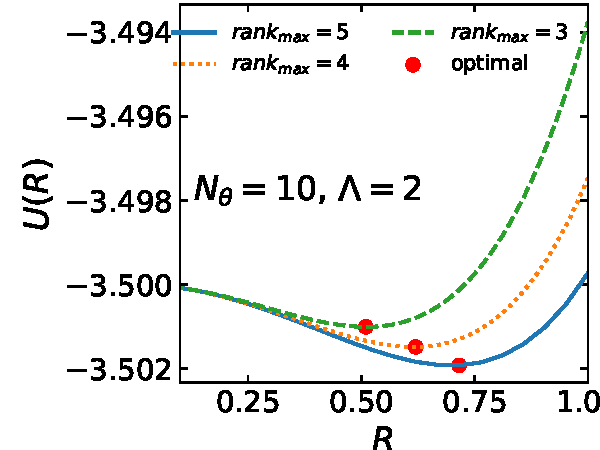
\includegraphics[width=0.6\textwidth]{SimplexUncertainty}}
\caption{\label{fig:SimplexUncertainty}
The integrated uncertainty for training with points set in a simplex geometry is found to depend only weakly on the radius. A Gaussian prior was assumed. The weak dependence was used to justify using a rather ad-hoc choice of radii for the simplex points, or as in the case of type 2, a second radius for the bisecting points.}
\end{figure}

One issue with the simplex is that the first set of $N+1$ training points would all be placed at the same radius. If the prior parameter distribution is uniform within an $N-$dimensional hyper cube, the training  points could be rather far from the corners in that space. Issues with such priors are discussed in the next section.

\subsection{The Pernicious Nature of Step-Function Priors in High Dimension}

For purely Gaussian priors, one can scale the prior parameter space to be spherically symmetric. Unfortunately, that is not true for step function priors (uniform within some range). In that case the best one can do (if the priors for each parameter are independent) is to scale the parameter space such that each parameter has the constraint, $-1<\theta_i<1$. If the number of parameters is $N$, the hyper-cube has $2N$ faces and $2^N$ corners, a face being defined as one parameter being $\pm 1$ while the others are zero, while a corner has each parameter either $\pm 1$. For 10 parameters, there are 1024 corners, and for 15 parameters there are 32678 corners. Thus, it might be untenable to place a training point in each corner. 

One can also see the problem with placing the training points in a spherically symmetric fashion as is done with the {\it Simplex Sampler}. The hyper-volume of the parameter-space hyper-cube is $2^N$, whereas the volume of an $N-$dimensional hyper-sphere of radius $R=1$ is 
\begin{align*}\eqnumber
V_{\rm sphere}=\Omega_N\int_0^R dr~r^{N-1}=\Omega_N\frac{R^N}{N}.
\end{align*}
The solid angle, $\Omega_N$ in $N$ dimensions is
\begin{align*}\eqnumber
\Omega_N&=\frac{2\pi^{N/2}}{\Gamma(N/2)},
\end{align*}
and after putting this together, the fraction of the hyper-cube's volume that is within the hyper-sphere is
\begin{align*}\eqnumber
\frac{V_{\rm sphere}}{V_{\rm cube}}&=\left\{\begin{array}{rl}
\frac{(\pi/2)^{N/2}}{N!!},&N=2,4,6,8\cdots\\
\frac{(\pi/2)^{(N-1)/2}}{N!!},&N=3,5,7,\cdots\end{array}\right.
\end{align*}
In two dimensions, the ratio is $\pi/4$, and in three dimensions it is $\pi/6$. In 10 dimensions it is $2.5\times 10^{-3}$. For high dimensions only a small fraction of the parameter space can ever lie inside inside a sphere used to place points. And, if the model is expensive, it may not be tenable to run the full model inside every corner. 

One can also appreciate the scope of the problem by considering the radius of the corners vs. the radius of  the sphere. The maximum value of $|\vec{\theta}|$ is $\sqrt{N}$. So, for 9 parameters, if the  training points were all located at positions $|\vec{\theta}|<1$, one would have to extrapolate all the way to $|\vec{\theta}|=3$. Thus, unless the model is exceptionally smooth, one needs to devise a strategy to isolate the portion of likely parameter space using some original set of full-model runs, then augment those runs in the likely region. 

A third handle for viewing the issue in $N$ dimensions is to compare the r.m.s. radii of the hyper-sphere to that of the hyper-cube. For the cube where each side has length $2a$,
\begin{align*}\eqnumber
\left(R_{\rm r.m.s.}^{\rm(cube)}\right)^2&=a^2\frac{N}{3}.
\end{align*}
whereas for a sphere of radius $a$,
\begin{align*}\eqnumber
\left(R_{\rm r.m.s.}^{\rm(sphere)}\right)^2&=a^2\frac{N+2}{N}.
\end{align*}
The ratio of the radii is then
\begin{align*}\eqnumber
\frac{R_{\rm r.m.s.}^{\rm(sphere)}}{R_{\rm r.m.s.}^{\rm(cube)}}&=\sqrt{\frac{3}{N+2}}.
\end{align*}
Thus, in 10 dimensions, if the training points are placed at a distance $a$ from the origin, the r.m.s. radii of the interior space would be half that of the entire space. Further, the r.m.s. radii of the points in the cube, $a\sqrt{N/3}$, would be about 83\% higher than the radius of the training points. 

Of course, these problems would be largely avoided if the number of parameters was a half dozen or fewer, or if one was confident that the function was extremely smooth. In the first two sections of this paper, the smoothness parameter, $\Lambda$, was set to a constant. There might be prior knowledge that certain parameters affect the observables only weakly. In that case, the response to these parameters can be considered as linear. This could be done by scaling those parameters so that they vary over a smaller range. If a parameter varies only between $-0.1$ and $0.1$, that effectively applies a smoothness parameter in those directions that is ten times higher. Unfortunately, the choice of which parameters to rescale in this fashion would likely vary depending on which observable is being emulated. Because all the observables might be calculated in a full model run, one needs to identify parameters that would likely have weak response on all observables. 

\section{Tests of {\it Smooth Emulator}}

Here, we show several results for testing {\it Smooth Emulator}. For these tests we consider a surrogate full-model generated from Taylor expansions with randomized coefficients, exactly according to the form assumed by the emulator. These functions are characterized by a smoothness parameter, $\Lambda$, a variance for the coefficients, $\sigma_A$, and a maximum rank. If the emulator works correctly, 68\% of the discrepancies in emulated functions, compared to the true model, should fall within one standard deviation. Performing the same test as described in the tutorial, Fig. \ref{fig:smoothtest_vsfullmodel} compares emulator predictions to 50 different surrogate models. Each surrogate model was constructed according to Taylor expansions with $\Lambda=3$, a maximum rank of 4, and $\sigma_A=100$. Although only 50 such models are illustrated here, this was attempted with 5000 models, and it was found that the percentage of predictions within one sigma was within a few tenths of a percent of the 68\% expected, thus validating both the emulator's prediction of both its value and its estimate of its uncertainty.
\begin{figure}
\centerline{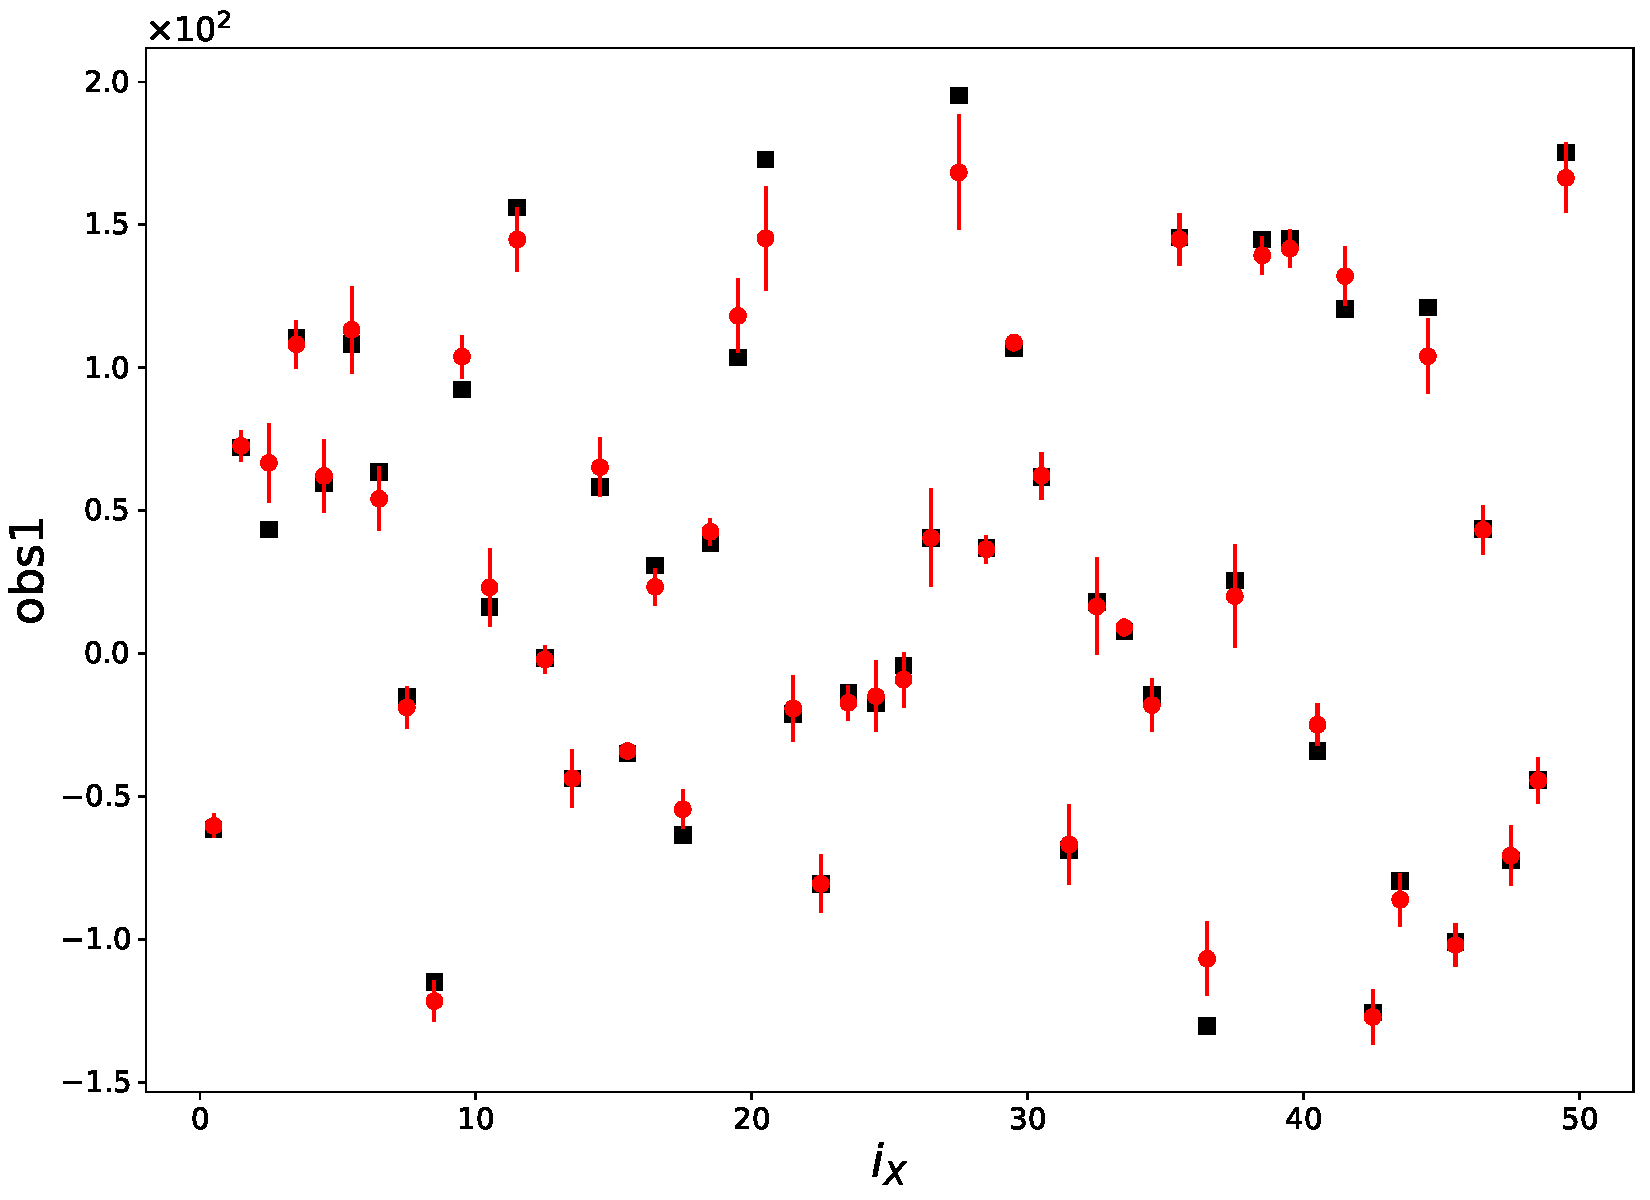
\includegraphics[width=0.6\textwidth]{YvsY_smooth}}
\caption{\label{fig:smoothtest_vsfullmodel}
Emulator predictions are compared to a surrogate model with Taylor expansions based on $\Lambda=3$ and $\sigma_A=100$. As can be seen approximately 68\% of the predictions were within one sigma of the true model, validating the emulator, both in regards to its predicted value and its uncertainty estimate.}
\end{figure}

Figure \ref{fig:vslambda} shows the average of surrogate-model predictions $\ln(Z)$, $\sigma_A$ and the percentage of predictions within one sigma over 500 instances. These are shown as a function of the emulator's $\Lambda$. Because the surrogate models were constructed with $\Lambda=3$, the value of $\ln(Z)$ should be a maximum there. Further, for $\Lambda=3$, the extracted value of $\sigma_A$ should be 100, and 68\% of emulator predictions should be within the emulator's uncertainty estimate. The emulator passes all these tests beautifully, but as can be seen, whereas the prediction of $\sigma_A$ is remarkably accurate, the value of $\ln(Z)$ is quite uncertain. Thus, finding $\Lambda$ for a given emulator might be problematic. Figure \ref{fig:logPinstances} shows $\ln(Z)$ for several individual models. This was repeated for 5, 10 and 15 parameters. For smaller numbers of parameters, using $\ln(Z)$ vs $\Lambda$ to determine $\Lambda$  is especially problematic. Thus, the User might want to simply fix $\Lambda$ at some value, e.g 2.5, and live with the consequences.

\begin{figure}
\parbox[t]{0.45\textwidth}{
\centerline{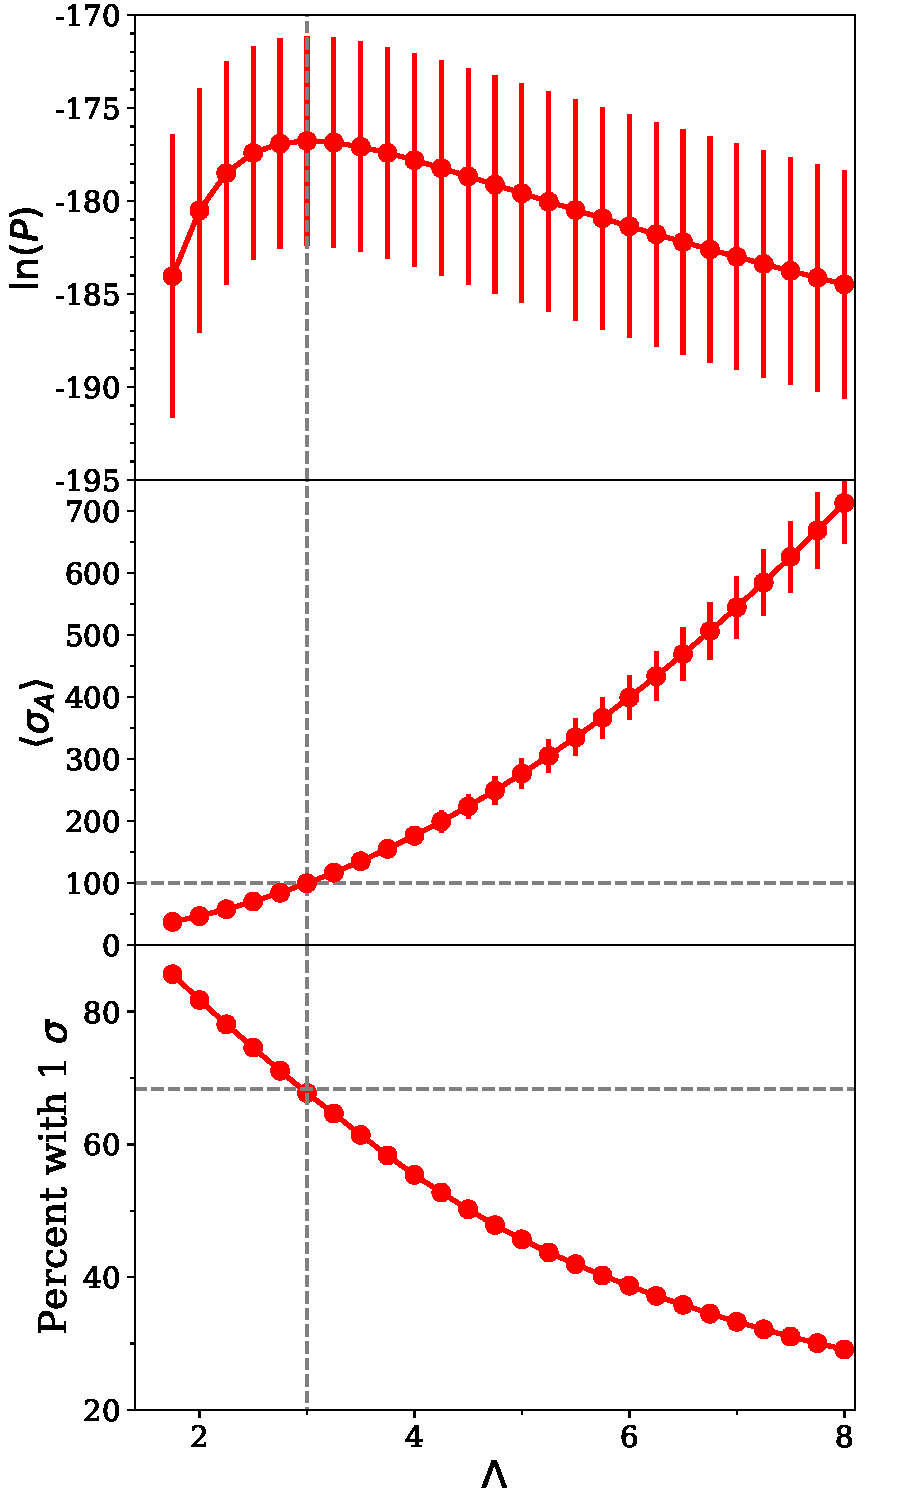
\includegraphics[width=0.45\textwidth]{vslambda}}
\caption{\label{fig:vslambda}
A ensemble of 5000 surrogate models, each generated with $\Lambda=3$ an $\sigma_A=100$ were emulated. The extracted values of $\ln(Z)$ an $\sigma_A$, along with the percentage of emulator predictions withing the emulator's uncertainty were plotted agains the value of $\Lambda$ assumed for the emulator. Indeed, for $\Lambda=3$, $\ln(Z)$ is at a maximum, $\sigma_A=100$ and 68\% of the predictions are within the estimated uncertainty. Unfortunately, $\ln(Z)$ has a high instance-to-instance variability.}}
~~~~\parbox[t]{0.45\textwidth}{ \vspace*{-266pt}
\centerline{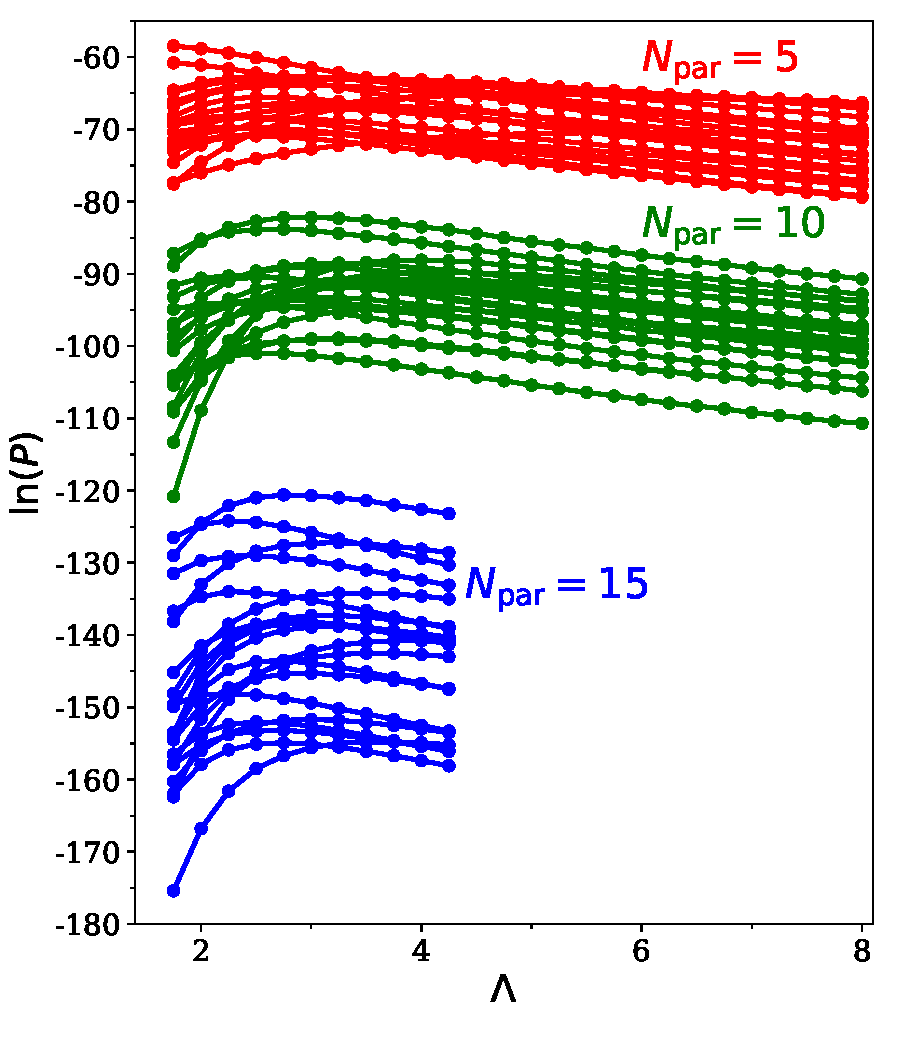
\includegraphics[width=0.45\textwidth]{logPinstances}}
\caption{\label{fig:logPinstances}
For 20 instances of the surrogate function, $\ln(Z)$ is plotted vs. $\Lambda$. Although if one were to average over thousands of surrogate models, one could extract $\Lambda$ accurately, the extraction is rather inaccurate on a model-by-model basis. This is especially true if the model has smaller numbers of parameters.}}
\end{figure}


\end{document}
